\documentclass[10pt]{article}

\usepackage[a4paper,margin=0.65in]{geometry}
\usepackage{amsmath,amssymb}
\usepackage{graphicx}
\usepackage{booktabs}
\usepackage{array}
\usepackage{float}
\usepackage{hyperref}
\usepackage{enumitem}
\usepackage{xcolor}
\usepackage{tikz}
\usetikzlibrary{positioning,arrows.meta,shapes.geometric,fit,calc}

\setlist{nosep,leftmargin=*}
\renewcommand{\arraystretch}{1.2}
\setlength{\parindent}{0pt}
\setlength{\parskip}{2pt}

\tikzset{
layer/.style={
draw,
rounded corners,
minimum width=1.7cm,
minimum height=0.65cm,
align=center,
fill=blue!10,
font=\scriptsize
},
smalllayer/.style={
draw,
rounded corners,
minimum width=1.35cm,
minimum height=0.58cm,
align=center,
fill=green!10,
font=\scriptsize
},
arrow/.style={
-{Latex[length=2mm]},
thin
}
}

\begin{document}

%%%%%%%%%%%%%%%%%%%%%%%%%%%%%%%%%%%%%%%%%%%%%%%%%%%%%%%%%%%%
% TITLE
%%%%%%%%%%%%%%%%%%%%%%%%%%%%%%%%%%%%%%%%%%%%%%%%%%%%%%%%%%%%

\begin{center}

{\large\textbf{Shiv Nadar University Chennai}}

\vspace{2mm}

{\normalsize\textbf{CS3807 -- Deep Learning Laboratory}}

\vspace{2mm}

{\large\textbf{Experiment 7}}

\vspace{1mm}

{\normalsize\textbf{End-to-End Study of Autoencoders, Convolutional}}

{\normalsize\textbf{Autoencoders, Denoising Autoencoders and Variational Autoencoders}}

\vspace{2mm}

{\normalsize Ankith U Davey \quad 24011101004}

\end{center}

\vspace{3mm}

\begin{tabular}{|p{3.4cm}|p{9.0cm}|p{1.4cm}|}
\hline
Degree \& Branch &
B.Tech Artificial Intelligence \& Data Science &
Semester V\\
\hline
Subject Code \& Name &
CS3807 -- Deep Learning Laboratory &
AY: 2026--27\\
\hline
\end{tabular}

%%%%%%%%%%%%%%%%%%%%%%%%%%%%%%%%%%%%%%%%%%%%%%%%%%%%%%%%%%%%
\section*{1. Objective}

The objective of this experiment is to develop an end-to-end understanding of
autoencoders and their variants for image representation, reconstruction,
denoising and generative modeling.

The experiment begins with a fully connected autoencoder, progresses to a
Convolutional Autoencoder (CAE), introduces image corruption for denoising,
and finally develops a Variational Autoencoder (VAE). Students will visualize
the learned latent representation, compare reconstruction quality using
quantitative and qualitative measures, and explore the generative capability
of the VAE.

The same image dataset and a controlled experimental protocol should be used
throughout the experiment wherever possible.

%%%%%%%%%%%%%%%%%%%%%%%%%%%%%%%%%%%%%%%%%%%%%%%%%%%%%%%%%%%%
\section*{2. Learning Outcomes}

After completing this experiment, students will be able to:

\begin{itemize}
\item explain the encoder--latent--decoder structure of an autoencoder;
\item prepare image data for reconstruction-based learning;
\item implement a fully connected autoencoder;
\item implement a Convolutional Autoencoder for image reconstruction;
\item introduce controlled noise and build a denoising autoencoder;
\item evaluate reconstruction using MSE, MAE and SSIM;
\item visualize and interpret latent representations;
\item explain the probabilistic latent representation of a VAE;
\item implement the reparameterization trick;
\item calculate and interpret reconstruction and KL-divergence losses;
\item generate new images by sampling from a learned latent space; and
\item compare deterministic and variational latent representations.
\end{itemize}

%%%%%%%%%%%%%%%%%%%%%%%%%%%%%%%%%%%%%%%%%%%%%%%%%%%%%%%%%%%%
\section*{3. Dataset and Experimental Setup}

\textbf{Dataset: MNIST Handwritten Digit Dataset}

MNIST contains grayscale images of handwritten digits from 0 to 9. Each image
has spatial dimensions

\[
28\times28\times1.
\]

The dataset is particularly suitable for this experiment because the images
are small, the classes have visually meaningful structure, and the same image
format can be directly supplied to fully connected, convolutional and
variational autoencoders.

The dataset can be loaded directly using Keras/TensorFlow:

\url{https://www.tensorflow.org/api_docs/python/tf/keras/datasets/mnist}

\textbf{Recommended laboratory subset:}

Use 10,000 training images and 2,000 test images for the main laboratory
execution. The full MNIST dataset may be used if computational resources
permit.

The labels are not required as reconstruction targets. The original image is
the target:

\[
\boxed{x\rightarrow \text{Encoder}\rightarrow z
\rightarrow\text{Decoder}\rightarrow\hat{x}}
\]

where $x$ is the input image and $\hat{x}$ is its reconstruction.

%%%%%%%%%%%%%%%%%%%%%%%%%%%%%%%%%%%%%%%%%%%%%%%%%%%%%%%%%%%%
\section*{4. Expected Input and Output}

\subsection*{Expected Input}

Each input image has shape

\[
28\times28\times1.
\]

For a batch of 32 images:

\[
X\in\mathbb{R}^{32\times28\times28\times1}.
\]

Pixel values should be converted from

\[
[0,255]\rightarrow[0,1].
\]

For a fully connected autoencoder, the image may be flattened:

\[
28\times28=784.
\]

Therefore,

\[
x\in\mathbb{R}^{784}.
\]

For a convolutional autoencoder, retain the spatial structure:

\[
x\in\mathbb{R}^{28\times28\times1}.
\]

\subsection*{Expected Output}

The primary output is a reconstructed image:

\[
\hat{x}\in\mathbb{R}^{28\times28\times1}.
\]

Students must display:

\begin{verbatim}
Original image
Reconstructed image
Reconstruction error
\end{verbatim}

For the denoising model, display:

\begin{verbatim}
Original clean image
Noisy image
Denoised reconstruction
\end{verbatim}

For the VAE, display newly generated samples obtained by sampling from the
latent distribution.

%%%%%%%%%%%%%%%%%%%%%%%%%%%%%%%%%%%%%%%%%%%%%%%%%%%%%%%%%%%%
\section*{5. Overall Experimental Pipeline}

The complete experiment follows:

\begin{center}
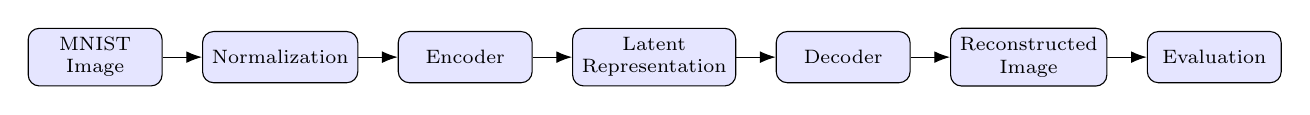
\begin{tikzpicture}[node distance=5mm]
\node[layer](a){MNIST\\Image};
\node[layer,right=of a](b){Normalization};
\node[layer,right=of b](c){Encoder};
\node[layer,right=of c](d){Latent\\Representation};
\node[layer,right=of d](e){Decoder};
\node[layer,right=of e](f){Reconstructed\\Image};
\node[layer,right=of f](g){Evaluation};

\foreach \x/\y in {a/b,b/c,c/d,d/e,e/f,f/g}
\draw[arrow](\x)--(\y);
\end{tikzpicture}
\end{center}

The experiment consists of four related studies:

\begin{enumerate}
\item Fully Connected Autoencoder
\item Convolutional Autoencoder
\item Denoising Convolutional Autoencoder
\item Variational Autoencoder
\end{enumerate}

%%%%%%%%%%%%%%%%%%%%%%%%%%%%%%%%%%%%%%%%%%%%%%%%%%%%%%%%%%%%
\section*{6. Source Code}

The complete source code, including the Jupyter notebook and all generated plots, is available in the accompanying GitHub repository:

\vspace{4pt}
\noindent\texttt{https://github.com/Ankith-Davey/Deep-Learning-Lab-Ankith-24011101004/tree/main/Lab\%207}    
\vspace{4pt}

%%%%%%%%%%%%%%%%%%%%%%%%%%%%%%%%%%%%%%%%%%%%%%%%%%%%%%%%%%%%
\section*{7. Exploring Autoencoders}

An autoencoder learns to reproduce its input at the output.

The encoder maps the input to a lower-dimensional representation:

\[
z=f_{\theta}(x),
\]

and the decoder reconstructs the input:

\[
\hat{x}=g_{\phi}(z).
\]

The training objective is to minimize reconstruction error:

\[
\mathcal{L}_{rec}
=
\frac{1}{N}\sum_{i=1}^{N}
\|x_i-\hat{x}_i\|^2.
\]

\begin{center}
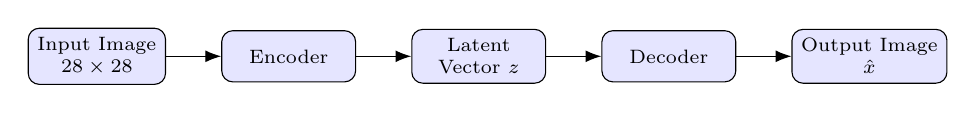
\begin{tikzpicture}[node distance=7mm]
\node[layer](a){Input Image\\$28\times28$};
\node[layer,right=of a](b){Encoder};
\node[layer,right=of b](c){Latent\\Vector $z$};
\node[layer,right=of c](d){Decoder};
\node[layer,right=of d](e){Output Image\\$\hat{x}$};

\foreach \x/\y in {a/b,b/c,c/d,d/e}
\draw[arrow](\x)--(\y);
\end{tikzpicture}
\end{center}

The latent vector is a compressed representation of the input.

%%%%%%%%%%%%%%%%%%%%%%%%%%%%%%%%%%%%%%%%%%%%%%%%%%%%%%%%%%%%
\section*{8. Fully Connected Autoencoder}

Flatten each image from

\[
28\times28=784
\]

to a vector of length 784.

Use the following architecture:

\begin{center}
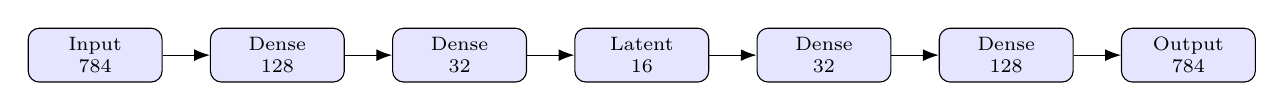
\begin{tikzpicture}[node distance=6mm]
\node[layer](a){Input\\784};
\node[layer,right=of a](b){Dense\\128};
\node[layer,right=of b](c){Dense\\32};
\node[layer,right=of c](d){Latent\\16};
\node[layer,right=of d](e){Dense\\32};
\node[layer,right=of e](f){Dense\\128};
\node[layer,right=of f](g){Output\\784};

\foreach \x/\y in {a/b,b/c,c/d,d/e,e/f,f/g}
\draw[arrow](\x)--(\y);
\end{tikzpicture}
\end{center}

Use ReLU activation in hidden layers and sigmoid activation in the output
layer.

\textbf{Suggested configuration:}

\begin{center}
\begin{tabular}{|l|l|}
\hline
Parameter & Value\\
\hline
Latent dimension & 16\\
Optimizer & Adam\\
Learning rate & $10^{-3}$\\
Batch size & 128\\
Epochs & 20\\
Loss & Binary Cross-Entropy\\
\hline
\end{tabular}
\end{center}

%%%%%%%%%%%%%%%%%%%%%%%%%%%%%%%%%%%%%%%%%%%%%%%%%%%%%%%%%%%%
\section*{9. Required Analysis of the Basic Autoencoder}

\textbf{Plot 1: Original versus Reconstructed Images}

\begin{figure}[H]
\centering
\includegraphics[width=0.95\textwidth]{01_fc_ae_original_vs_reconstructed.png}
\caption{FC-AE reconstructions on 10 test images. Top row: original. Bottom row: reconstructed.}
\end{figure}

\textbf{Inference:} The fully connected auto encoder preserves the overall shape of most digits but the plot indicates that since there are only 16 latent values per image, a few of the details are lost. The edges appear to be blurred, especially for the curved digits. The first 5 in the test batch is reconstructed as closer to a 6. This is because of the compressing of the image into 16 values does not learn enough features to fully reconstruct a digit.

\textbf{Plot 2: Training and Validation Reconstruction Loss}

\begin{figure}[H]
\centering
\includegraphics[width=0.6\textwidth]{02_fc_ae_train_val_loss.png}
\caption{FC-AE training vs validation loss across 20 epochs.}
\end{figure}

\textbf{Inference:} Both the training and validation loss  decrease gradually and flatten out by the final epoch, with the validation loss remaining slightly below training loss throughout. This indicates that the model does not overfit and this could further improve with more number of epochs.

%%%%%%%%%%%%%%%%%%%%%%%%%%%%%%%%%%%%%%%%%%%%%%%%%%%%%%%%%%%%
\section*{10. Reconstruction Metrics}

Students must calculate the following metrics on the test set.

\subsection*{Mean Squared Error}

\[
MSE=
\frac{1}{N}
\sum_{i=1}^{N}
(x_i-\hat{x}_i)^2.
\]

\subsection*{Mean Absolute Error}

\[
MAE=
\frac{1}{N}
\sum_{i=1}^{N}
|x_i-\hat{x}_i|.
\]

\subsection*{Structural Similarity}

Calculate SSIM between the original and reconstructed images.

The implementation may use:

\url{https://scikit-image.org/docs/stable/api/skimage.metrics.html}

Report:

\begin{center}
\begin{tabular}{|l|c|}
\hline
Metric & Value\\
\hline
Test MSE & 0.02252\\
Test MAE & 0.05972\\
Mean SSIM & 0.7452\\
\hline
\end{tabular}
\end{center}

%%%%%%%%%%%%%%%%%%%%%%%%%%%%%%%%%%%%%%%%%%%%%%%%%%%%%%%%%%%%
\section*{11. Convolutional Autoencoder}

A Convolutional Autoencoder preserves spatial structure and uses convolutional
operations in the encoder and upsampling/transposed convolution operations
in the decoder.

The conceptual architecture is:

\begin{center}
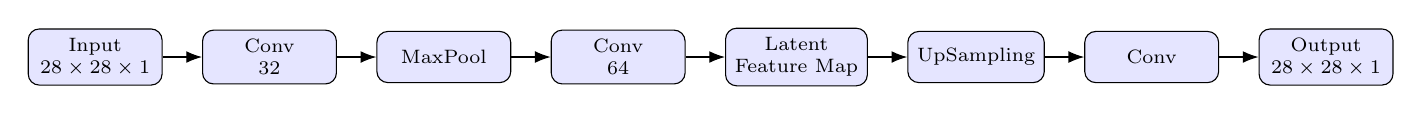
\begin{tikzpicture}[node distance=5mm]
\node[layer](a){Input\\$28\times28\times1$};
\node[layer,right=of a](b){Conv\\32};
\node[layer,right=of b](c){MaxPool};
\node[layer,right=of c](d){Conv\\64};
\node[layer,right=of d](e){Latent\\Feature Map};
\node[layer,right=of e](f){UpSampling};
\node[layer,right=of f](g){Conv};
\node[layer,right=of g](h){Output\\$28\times28\times1$};

\foreach \x/\y in {a/b,b/c,c/d,d/e,e/f,f/g,g/h}
\draw[arrow](\x)--(\y);
\end{tikzpicture}
\end{center}

A possible implementation is:

\begin{verbatim}
Input(28,28,1)
Conv2D(32, 3, activation='relu', padding='same')
MaxPooling2D(2, padding='same')
Conv2D(64, 3, activation='relu', padding='same')
MaxPooling2D(2, padding='same')
Conv2D(64, 3, activation='relu', padding='same')
UpSampling2D(2)
Conv2D(32, 3, activation='relu', padding='same')
UpSampling2D(2)
Conv2D(1, 3, activation='sigmoid', padding='same')
\end{verbatim}

The exact implementation may use Conv2DTranspose instead of UpSampling2D.

%%%%%%%%%%%%%%%%%%%%%%%%%%%%%%%%%%%%%%%%%%%%%%%%%%%%%%%%%%%%
\section*{12. Comparing Fully Connected and Convolutional Autoencoders}

Both models were trained using the same 10,000 training images and evaluated on the same 2,000 test images.

\begin{center}
\begin{tabular}{|l|c|c|c|c|}
\hline
Model & MSE & MAE & SSIM & Parameters\\
\hline
Fully Connected AE & 0.02252 & 0.05972 & 0.7452 & 211{,}040\\
Convolutional AE (UpSampling) & 0.00246 & 0.01502 & 0.9751 & 74{,}497\\
\hline
\end{tabular}
\end{center}

\textbf{Plot 3: Reconstruction Comparison}

\begin{figure}[H]
\centering
\includegraphics[width=0.95\textwidth]{03_fc_vs_cae_reconstruction.png}
\caption{Original (top) vs FC-AE reconstruction (middle) vs CAE reconstruction (bottom).}
\end{figure}

\textbf{Inference:} The convolutional auto-encoder outperforms the fully connected auto encoder by a wide margin on every metric, around 9 times lower MSE and 0.23 higher SSIM, while still using less than half the parameters. This is due to preservation of spatial structure by CNNs where in it operates on local neighborhoods of pixels rather than flattening the image, so edges and strokes are reconstructed in a more better way. The CAE row in the image is nearly indistinguishable from the original in most cases, while the FC-AE row stays visibly blurred, including the same 5-to-6 misclassification observed in Plot 1. This shows convolutional structure is a much more efficient way to encode image data than a flat dense bottleneck, both in reconstruction quality and in parameter cost.

\textbf{Additional Exercise 4: Conv2DTranspose vs UpSampling Decoder}

The CAE decoder was rebuilt using \texttt{Conv2DTranspose} layers in place of \texttt{UpSampling2D} + \texttt{Conv2D}, keeping the same filter counts and depth.

\begin{center}
\begin{tabular}{|l|c|c|c|c|}
\hline
Decoder Type & MSE & MAE & SSIM & Parameters\\
\hline
UpSampling2D & 0.00246 & 0.01502 & 0.9751 & 74{,}497\\
Conv2DTranspose & 0.00224 & 0.01402 & 0.9779 & 83{,}745\\
\hline
\end{tabular}
\end{center}

\begin{figure}[H]
\centering
\includegraphics[width=0.95\textwidth]{ex4_upsampling_vs_transpose.png}
\caption{Original vs UpSampling decoder vs Conv2DTranspose decoder.}
\end{figure}

\textbf{Inference:} The Conv2DTranspose decoder performs marginally better on every metric, at the cost of roughly 9{,}000 additional parameters from the learned upsampling filters. The difference in the reconstructions is barely visible because both the rows look similar to the original. This is also because UpSampling2D is a fixed, non-learned interpolation while Conv2DTranspose learns how to upsample, giving it slightly more flexibility. For a dataset as simple as MNIST, this extra flexibility only produces a small improvement, but it may matter more on higher-resolution or more complex images.

%%%%%%%%%%%%%%%%%%%%%%%%%%%%%%%%%%%%%%%%%%%%%%%%%%%%%%%%%%%%
\section*{13. Denoising Autoencoder}

A denoising autoencoder receives a corrupted image but is trained to
reconstruct the original clean image.

The training mapping is:

\[
\boxed{\tilde{x}\rightarrow\text{Encoder}\rightarrow z
\rightarrow\text{Decoder}\rightarrow\hat{x}}
\]

where $\tilde{x}$ is a noisy version of the clean image $x$.

\begin{center}
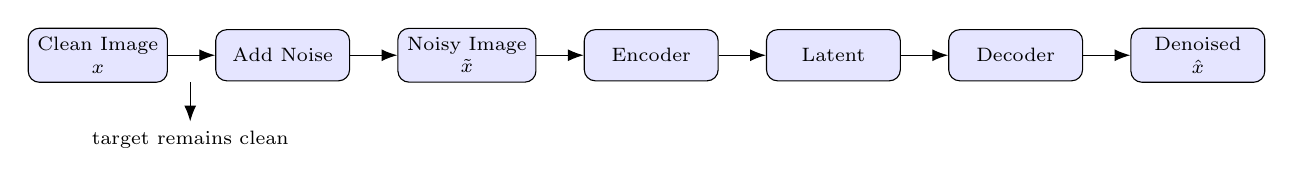
\begin{tikzpicture}[node distance=6mm]
\node[layer](a){Clean Image\\$x$};
\node[layer,right=of a](b){Add Noise};
\node[layer,right=of b](c){Noisy Image\\$\tilde{x}$};
\node[layer,right=of c](d){Encoder};
\node[layer,right=of d](e){Latent};
\node[layer,right=of e](f){Decoder};
\node[layer,right=of f](g){Denoised\\$\hat{x}$};

\foreach \x/\y in {a/b,b/c,c/d,d/e,e/f,f/g}
\draw[arrow](\x)--(\y);

\draw[arrow]($(a.south)!0.5!(b.south)$) -- ++(0,-5mm)
node[below,font=\scriptsize]{target remains clean};
\end{tikzpicture}
\end{center}

%%%%%%%%%%%%%%%%%%%%%%%%%%%%%%%%%%%%%%%%%%%%%%%%%%%%%%%%%%%%
\section*{14. Adding Image Noise}

Use at least two corruption types.

\subsection*{Gaussian Noise}

\[
\tilde{x}=x+n,
\qquad
n\sim\mathcal{N}(0,\sigma^2).
\]

Suggested standard deviations:

\[
\sigma\in\{0.1,0.2,0.3\}.
\]

Clip the resulting image to the range $[0,1]$.

\subsection*{Salt-and-Pepper Noise}

Randomly replace a small proportion of pixels with values close to 0 or 1.

Suggested corruption levels:

\[
p\in\{0.05,0.10,0.20\}.
\]

%%%%%%%%%%%%%%%%%%%%%%%%%%%%%%%%%%%%%%%%%%%%%%%%%%%%%%%%%%%%
\section*{15. Required Denoising Plots}

\textbf{Plot 4: Clean vs. Noisy vs. Denoised}

\begin{figure}[H]
\centering
\includegraphics[width=0.95\textwidth]{04_denoising_clean_noisy_denoised.png}
\caption{Clean (top) vs Gaussian noisy, $\sigma=0.2$ (middle) vs denoised (bottom).}
\end{figure}

\textbf{Plot 5: Noise Level vs. Reconstruction Quality (Gaussian)}

\begin{center}
\begin{tabular}{|c|c|c|c|}
\hline
Noise Level ($\sigma$) & MSE & MAE & SSIM\\
\hline
0.1 & 0.00299 & 0.01683 & 0.9666\\
0.2 & 0.00438 & 0.02087 & 0.9489\\
0.3 & 0.00638 & 0.02588 & 0.9236\\
\hline
\end{tabular}
\end{center}

\begin{figure}[H]
\centering
\includegraphics[width=0.95\textwidth]{05_noise_level_vs_quality.png}
\caption{MSE, MAE, and SSIM vs Gaussian noise standard deviation.}
\end{figure}

\textbf{Inference:} As the Gaussian noise level increases from $\sigma=0.1$ to $\sigma=0.3$, MSE and MAE both increase steadily while SSIM drops from about 0.967 to 0.924. This is expected, since a higher standard deviation corrupts more pixels more severely, giving the encoder a noisier signal to work with. But the drop in SSIM is fairly small even at the highest noise level, and Plot 4 confirms visually that the denoised digits stay recognizable and close to the clean originals throughout. This shows the denoising CAE is able to recover the major structure of the digit even under fairly heavy corruption, though fine strokes and edges do get a little softer as noise increases.

\textbf{Additional Exercise 2 \& 3: Gaussian vs Salt-and-Pepper Noise Comparison}

\begin{center}
\begin{tabular}{|c|c|c|c|c|}
\hline
Noise Type & Level & MSE & MAE & SSIM\\
\hline
Gaussian & $\sigma=0.1$ & 0.00299 & 0.01683 & 0.9666\\
Gaussian & $\sigma=0.2$ & 0.00438 & 0.02087 & 0.9489\\
Gaussian & $\sigma=0.3$ & 0.00638 & 0.02588 & 0.9236\\
Salt-Pepper & $p=0.05$ & 0.00378 & 0.01844 & 0.9598\\
Salt-Pepper & $p=0.10$ & 0.00458 & 0.02056 & 0.9497\\
Salt-Pepper & $p=0.20$ & 0.00718 & 0.02726 & 0.9179\\
\hline
\end{tabular}
\end{center}

\begin{figure}[H]
\centering
\includegraphics[width=0.95\textwidth]{ex2_gaussian_vs_saltpepper.png}
\caption{Clean vs Gaussian-noisy vs Gaussian-denoised vs Salt-Pepper-denoised.}
\end{figure}

\textbf{Inference:} At matched moderate severity (Gaussian $\sigma=0.2$ vs Salt-Pepper $p=0.10$), both noise types give nearly identical SSIM (0.9489 vs 0.9497), so neither is clearly harder to denoise at this level. At the highest corruption levels tested, salt-and-pepper (SSIM 0.9179 at $p=0.20$) degrades slightly more than Gaussian (SSIM 0.9236 at $\sigma=0.3$), which is expected as salt-and-pepper replaces pixels outright with 0 or 1 rather than adding a smaller perturbation, so a badly corrupted pixel carries no information about the original value at all. Visually, both the denoised rows in the figure look close to the clean digits, so the CAE is fairly robust to both types of corruption on this dataset.

%%%%%%%%%%%%%%%%%%%%%%%%%%%%%%%%%%%%%%%%%%%%%%%%%%%%%%%%%%%%
\section*{16. Variational Autoencoder}

A conventional autoencoder maps an input to a deterministic latent vector:

\[
z=f(x).
\]

A VAE instead learns a probability distribution:

\[
q_{\phi}(z|x)
=
\mathcal{N}
\left(
\mu(x),
\operatorname{diag}(\sigma^2(x))
\right).
\]

The encoder produces:

\[
\mu,\qquad \log\sigma^2.
\]

A latent vector is sampled using the reparameterization trick:

\[
z=\mu+\sigma\odot\epsilon,
\qquad
\epsilon\sim\mathcal{N}(0,I).
\]

\begin{center}
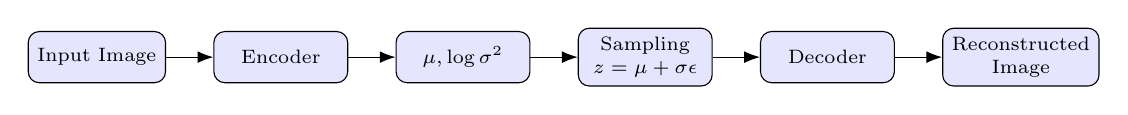
\begin{tikzpicture}[node distance=6mm]
\node[layer](a){Input Image};
\node[layer,right=of a](b){Encoder};
\node[layer,right=of b](c){$\mu,\log\sigma^2$};
\node[layer,right=of c](d){Sampling\\$z=\mu+\sigma\epsilon$};
\node[layer,right=of d](e){Decoder};
\node[layer,right=of e](f){Reconstructed\\Image};

\foreach \x/\y in {a/b,b/c,c/d,d/e,e/f}
\draw[arrow](\x)--(\y);
\end{tikzpicture}
\end{center}

%%%%%%%%%%%%%%%%%%%%%%%%%%%%%%%%%%%%%%%%%%%%%%%%%%%%%%%%%%%%
\section*{17. VAE Loss Function}

The VAE objective consists of two components.

\subsection*{Reconstruction Loss}

\[
\mathcal{L}_{rec}
=
-\mathbb{E}_{q_{\phi}(z|x)}
[\log p_{\theta}(x|z)].
\]

For normalized MNIST images, binary cross-entropy can be used.

\subsection*{KL Divergence}

\[
D_{KL}
\left(
q_{\phi}(z|x)\parallel p(z)
\right)
=
-\frac{1}{2}
\sum_j
\left(
1+\log\sigma_j^2-\mu_j^2-\sigma_j^2
\right).
\]

The total loss is

\[
\boxed{
\mathcal{L}_{VAE}
=
\mathcal{L}_{rec}
+
\mathcal{L}_{KL}
}
\]

where the prior is usually

\[
p(z)=\mathcal{N}(0,I).
\]

%%%%%%%%%%%%%%%%%%%%%%%%%%%%%%%%%%%%%%%%%%%%%%%%%%%%%%%%%%%%
\section*{18. VAE Implementation}

Use a small latent space so that it can be visualized.

Suggested latent dimension:

\[
z\in\mathbb{R}^{2}.
\]

The encoder should produce:

\[
\mu\in\mathbb{R}^{2},
\qquad
\log\sigma^2\in\mathbb{R}^{2}.
\]

The decoder maps

\[
z\rightarrow28\times28\times1.
\]

A compact architecture is:

\begin{center}
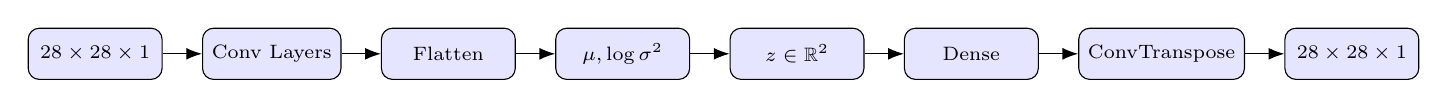
\begin{tikzpicture}[node distance=5mm]
\node[layer](a){$28\times28\times1$};
\node[layer,right=of a](b){Conv Layers};
\node[layer,right=of b](c){Flatten};
\node[layer,right=of c](d){$\mu,\log\sigma^2$};
\node[layer,right=of d](e){$z\in\mathbb{R}^2$};
\node[layer,right=of e](f){Dense};
\node[layer,right=of f](g){ConvTranspose};
\node[layer,right=of g](h){$28\times28\times1$};

\foreach \x/\y in {a/b,b/c,c/d,d/e,e/f,f/g,g/h}
\draw[arrow](\x)--(\y);
\end{tikzpicture}
\end{center}

%%%%%%%%%%%%%%%%%%%%%%%%%%%%%%%%%%%%%%%%%%%%%%%%%%%%%%%%%%%%
\section*{19. Exploring the VAE Latent Space}

Since the latent dimension is two, the encoded test images can be visualized directly in a two-dimensional plane. Labels are used only for coloring the plot; they were not supplied to the VAE during training.

\textbf{Plot 6: VAE Latent Space}

\begin{figure}[H]
\centering
\includegraphics[width=0.7\textwidth]{06_vae_latent_space.png}
\caption{VAE (latent dim=2) encoded test set, colored by digit label.}
\end{figure}

\textbf{Inference:} Two digits form clearly separated clusters on the outskirts of the plot . The remaining eight digits, however, pile into one dense, overlapping region near the center with no clear boundaries between them. This makes sense given a latent space of only 2 dimensions and 10 classes to represent, there is not enough room to separate every digit cleanly, so only the most visually distinct digits (0 and 1, which have very different stroke shapes from the rest) end up isolated, while visually similar digits like 3/5/8/9 blend together.

\textbf{Additional Exercise 5: VAE with Latent Dimension 8}

A second VAE was trained with latent dimension 8 instead of 2. Since an 8-dimensional space cannot be plotted directly, the encoded means were projected to 2D using PCA for a qualitative comparison only; this projected view is not one of the manual's required plots.

\begin{center}
\begin{tabular}{|l|c|c|c|c|c|}
\hline
VAE Config & MSE & MAE & SSIM & Recon. Loss & KL Loss\\
\hline
latent=2 & 0.04475 & 0.10482 & 0.5007 & 150.06 & 5.44\\
latent=8 & 0.02135 & 0.05606 & 0.7737 & 101.72 & 16.51\\
\hline
\end{tabular}
\end{center}

\begin{figure}[H]
\centering
\includegraphics[width=0.95\textwidth]{ex5_vae_latent2_vs_latent8.png}
\caption{Native 2D latent space (left) vs PCA-projected 8D latent space (right).}
\end{figure}

\textbf{Inference:} The latent dimension 8 VAE reconstructs noticeably better than latent dimension 2 on every metric, MSE nearly halves and SSIM rises from 0.50 to 0.77, since 8 dimensions can hold much more information about each digit than 2 can. Interestingly, the PCA-projected view of the 8D latent space does not look more separated than the native 2D space, if anything the digit clusters look more mixed after projection. This is not a contradiction because reconstruction quality and how cleanly a space separates on a 2D scatter are different things, and projecting 8 dimensions down to 2 for visualization necessarily discards information, which is the information that the extra 6 dimensions uses to hold. So the real benefit of the larger latent space is in reconstruction fidelity, not in how it happens to look when squeezed onto a 2D plot.

\textbf{Additional Exercise 6: Effect of Increasing the KL-Loss Contribution ($\beta$-VAE)}

The latent dimension 2 VAE was retrained with the KL term scaled by $\beta \in \{0.5, 1.0, 5.0\}$ to observe the reconstruction/regularization trade-off directly.

\begin{center}
\begin{tabular}{|c|c|c|c|c|}
\hline
$\beta$ & MSE & SSIM & Recon. Loss & KL Loss\\
\hline
0.5 & 0.04346 & 0.5133 & 147.27 & 6.78\\
1.0 & 0.04475 & 0.5007 & 150.06 & 5.44\\
5.0 & 0.04856 & 0.4614 & 161.27 & 3.04\\
\hline
\end{tabular}
\end{center}

\begin{figure}[H]
\centering
\includegraphics[width=0.95\textwidth]{ex6_beta_vae_latent_space.png}
\caption{VAE latent space at $\beta=0.5$, $\beta=1.0$, and $\beta=5.0$.}
\end{figure}

\textbf{Inference:} As $\beta$ increases, reconstruction loss rises steadily (147 to 161) while KL loss falls (6.78 to 3.04), which is exactly the trade-off a $\beta$-VAE is expected to show, a larger $\beta$ pushes the encoder harder toward matching the standard normal prior, at the cost of reconstruction accuracy. The latent space plots confirm this visually: at $\beta=5.0$ the points are noticeably more compressed toward the origin, and the two previously separated clusters (digits 0 and 1) pull inward and blend more with the central mass. This matches the theory directly, a stronger KL penalty regularizes the latent space more aggressively, making it more prior-like but less informative for reconstruction.

%%%%%%%%%%%%%%%%%%%%%%%%%%%%%%%%%%%%%%%%%%%%%%%%%%%%%%%%%%%%
\section*{20. Generating New Images with the VAE}

25 latent vectors were sampled from $z\sim\mathcal{N}(0,I)$ and passed through the decoder (latent dimension 2, $\beta=1.0$ model).

\textbf{Plot 7: Randomly Generated Images}

\begin{figure}[H]
\centering
\includegraphics[width=0.55\textwidth]{07_vae_generated_samples.png}
\caption{25 randomly generated samples from the VAE decoder.}
\end{figure}

\textbf{Inference:} The generated samples do resemble handwritten digits overall, and there is visible variation in stroke thickness and shape across the grid. However, this matches the latent space plot directly: samples in regions corresponding to the separated clusters (near where 0 and 1 sit in Plot 6) come out sharp and clearly recognizable, while samples drawn from the crowded central region often come out ambiguous, several look like they could plausibly be a 3, 5, 8, or 9 depending on how you read them. This is expected, since the decoder is essentially interpolating whatever digit classes overlap in that region of latent space, so a random draw there produces a blend rather than a single clean digit.

\textbf{Additional Exercise 7: Larger Sample Grid (100 samples)}

\begin{figure}[H]
\centering
\includegraphics[width=0.6\textwidth]{ex7_vae_100_samples.png}
\caption{100 randomly generated VAE samples.}
\end{figure}

\textbf{Inference:} At 100 samples the same pattern from the 25-sample grid holds and becomes clearer: clean, confidently-shaped digits (0s, 1s, straight strokes) appear reliably, but the majority of the grid is dominated by ambiguous shapes hovering between 5, 6, 8, and 9. This larger sample size does not really reveal new digit shapes beyond what the 25-sample grid already showed, it mainly confirms that the crowded central region of the latent space, rather than being a rare edge case, is actually where most of the probability mass of the standard normal prior falls, so most random samples land there rather than in the cleanly separated regions.

%%%%%%%%%%%%%%%%%%%%%%%%%%%%%%%%%%%%%%%%%%%%%%%%%%%%%%%%%%%%
\section*{21. Latent Space Interpolation}

Two test images were selected (a 3 and an 8) and their encoded latent means $z_A$, $z_B$ were interpolated using $z(\alpha) = (1-\alpha)z_A + \alpha z_B$ for $\alpha = 0, 0.1, \ldots, 1.0$, and every interpolated vector was decoded.

\textbf{Plot 8: Latent Space Interpolation}

\begin{figure}[H]
\centering
\includegraphics[width=0.95\textwidth]{08_vae_latent_interpolation.png}
\caption{Decoded images along the interpolation path from a test digit 3 to a test digit 8.}
\end{figure}

\textbf{Inference:} The decoded image barely changes across the entire interpolation path, it stays a 3-like shape throughout, with only a slight thickening of the loop around the midpoint. This is not really a case of a smooth transition between two different digits, it looks more like the two selected test points happen to sit close together in latent space, so moving between them does not cross much visual distance at all. This is expected because individual test samples of 3 and 8 can sit near each other in the crowded central region of the latent space even though their class centroids are further apart, so a single arbitrary pair of points is not guaranteed to interpolate across a large or meaningful stretch of the space.

\textbf{Additional Exercise 8: Targeted Digit-Region Interpolation}

Rather than picking two arbitrary test points, the per-digit centroid was computed for each of the 10 classes, and the pair with the largest Euclidean distance between centroids was selected for interpolation. This turned out to be digit 0 and digit 1 (distance $\approx 3.907$ in latent space).

\begin{figure}[H]
\centering
\includegraphics[width=0.95\textwidth]{ex8_centroid_interpolation.png}
\caption{Decoded images interpolating between the digit-0 centroid and the digit-1 centroid.}
\end{figure}

\textbf{Inference:} This interpolation shows a much clearer and more gradual transformation than the digit 3-to-8 interpolation above: the 0 opens up and thins out, briefly passes through shapes resembling 6 and 5, then straightens into a 1 by the final frame. This works because digits 0 and 1 sit at the two most separated ends of the latent space, so interpolating between their centroids actually traverses the full width of the space, unlike the arbitrary point pair used earlier. Taken together, these two interpolation results suggest that the smoothness of a VAE's interpolation depends heavily on which two points are chosen, and that centroid-based selection gives a much better sense of how the space is organized than an arbitrary pair of samples.

%%%%%%%%%%%%%%%%%%%%%%%%%%%%%%%%%%%%%%%%%%%%%%%%%%%%%%%%%%%%
\section*{22. Reconstruction Comparison Across Models}

\begin{center}
\begin{tabular}{|l|c|c|c|c|}
\hline
Model & MSE & MAE & SSIM & Parameters\\
\hline
Fully Connected AE & 0.02252 & 0.05972 & 0.7452 & 211{,}040\\
Convolutional AE (UpSampling) & 0.00246 & 0.01502 & 0.9751 & 74{,}497\\
Denoising CAE (Gaussian $\sigma=0.2$) & 0.00438 & 0.02087 & 0.9489 & 74{,}497\\
\hline
\end{tabular}
\end{center}

For the VAE, its reconstruction loss is reported separately because its total
objective also contains the KL-divergence term.

\begin{center}
\begin{tabular}{|l|c|}
\hline
VAE Metric (latent=2) & Value\\
\hline
Reconstruction Loss & 150.06\\
KL Loss & 5.44\\
Total Loss & 155.50\\
Test MSE & 0.04475\\
Test MAE & 0.10482\\
Mean SSIM & 0.5007\\
\hline
\end{tabular}
\end{center}

\textbf{Inference:} Across all four models, the CAE and its denoising variant clearly outperform both the FC-AE and the VAE on raw reconstruction quality, since they preserve spatial structure. The plain VAE (latent=2) has the weakest reconstruction of all four, which is expected -- it is deliberately constrained to a small, regularized latent space so it can be visualized and sampled from, trading some reconstruction accuracy for that generative capability. This is the fundamental difference between deterministic autoencoders, which are optimized purely for reconstruction, and the VAE, which balances reconstruction against a structured, samplable latent space.

\textbf{Plot 9: Training and Validation Loss for the VAE}

\begin{figure}[H]
\centering
\includegraphics[width=0.95\textwidth]{09_vae_train_val_loss.png}
\caption{VAE (latent=2) training vs validation loss, split into total loss, reconstruction loss, and KL divergence loss.}
\end{figure}

\textbf{Inference:} Total loss and reconstruction loss both decrease steadily over the 20 epochs and are close to flat by the end, with training and validation curves tracking each other closely throughout, so there is no sign of overfitting here either. The KL loss behaves quite differently, it actually increases steadily across training, from close to 0 at the start up to about 5.4 by the final epoch, and is still trending upward when training stops rather than having flattened out. This makes sense given how the two loss terms interact: early in training the encoder focuses on getting reconstruction loss down, which pulls the latent distributions away from the prior, and only later does the KL term start meaningfully pushing back. The reconstruction loss dominates the total loss by a wide margin throughout (around 150 versus around 5 for KL by the final epoch), which is expected given the loss weighting used ($\beta=1.0$), and explains why the VAE's MSE and SSIM values, while worse than the deterministic autoencoders, are still respectable rather than random.

%%%%%%%%%%%%%%%%%%%%%%%%%%%%%%%%%%%%%%%%%%%%%%%%%%%%%%%%%%%%

%%%%%%%%%%%%%%%%%%%%%%%%%%%%%%%%%%%%%%%%%%%%%%%%%%%%%%%%%%%%
\section*{23. Reconstruction Error Distribution}

The per-image reconstruction error was computed for the FC-AE on all 2,000 test images.

\textbf{Plot 9: Distribution of Reconstruction Errors}

\begin{figure}[H]
\centering
\includegraphics[width=0.75\textwidth]{09b_reconstruction_error_distribution.png}
\caption{Histogram of per-image reconstruction error (MSE) on the FC-AE test set.}
\end{figure}

\textbf{Inference:} The typical reconstruction error falls between about 0.002 and 0.07, with a mean of 0.0225 and standard deviation of 0.0112. The distribution is right-skewed, most images cluster in the 0.01 to 0.03 range, with a long thin tail extending out toward 0.07 representing a small number of much harder samples. This shape makes sense given the FC-AE's fixed 16-dimensional bottleneck, most digits are common enough shapes that the network reconstructs them reasonably well, but a handful of unusually written or ambiguous digits push the error much higher, forming the tail.

%%%%%%%%%%%%%%%%%%%%%%%%%%%%%%%%%%%%%%%%%%%%%%%%%%%%%%%%%%%%
\section*{24. Required High-Error Image Analysis}

\begin{center}
\begin{tabular}{|c|c|c|}
\hline
Sample & True Label & Reconstruction Error (MSE)\\
\hline
1 & 8 & 0.0713\\
2 & 0 & 0.0629\\
3 & 2 & 0.0608\\
4 & 5 & 0.0607\\
5 & 2 & 0.0597\\
\hline
\end{tabular}
\end{center}

\begin{figure}[H]
\centering
\includegraphics[width=0.95\textwidth]{10_high_error_samples.png}
\caption{The five FC-AE test reconstructions with the highest per-image MSE.}
\end{figure}

\textbf{Inference:} All five of the highest-error samples are, by eye, genuinely unusual or messy examples of handwriting -- the 8 has an oddly proportioned loop, the two 2s are drawn with an unconventional tail and shape, and the last one in particular barely reads as a 2 even to a human viewer. In every case, the FC-AE's reconstruction fails to preserve the digit's identity: the 8 comes out looking like a 4, one 2 turns into something closer to a 7, and the least legible original collapses into an unrecognizable blob. This suggests the FC-AE's 16-dimensional bottleneck has effectively learned a small set of "typical" digit templates, and images that deviate noticeably from typical handwriting get pulled toward the nearest template rather than reconstructed faithfully.

%%%%%%%%%%%%%%%%%%%%%%%%%%%%%%%%%%%%%%%%%%%%%%%%%%%%%%%%%%%%
\section*{25. Consolidated Results}

\begin{center}
\begin{tabular}{|l|c|c|c|c|c|}
\hline
Model & MSE & MAE & SSIM & Parameters & Time (s)\\
\hline
FC Autoencoder & 0.02252 & 0.05972 & 0.7452 & 211{,}040 & 11.5\\
Conv. Autoencoder (UpSampling) & 0.00246 & 0.01502 & 0.9751 & 74{,}497 & 19.5\\
Conv. Autoencoder (Conv2DTranspose) & 0.00224 & 0.01402 & 0.9779 & 83{,}745 & 19.1\\
Denoising CAE (Gaussian $\sigma=0.2$) & 0.00438 & 0.02087 & 0.9489 & 74{,}497 & 17.2\\
Denoising CAE (Salt-Pepper $p=0.10$) & 0.00458 & 0.02056 & 0.9497 & 74{,}497 & 17.3\\
VAE (latent=2) & 0.04475 & 0.10482 & 0.5007 & 284{,}933 & 21.7\\
VAE (latent=8) & 0.02135 & 0.05606 & 0.7737 & 304{,}529 & 21.1\\
\hline
\end{tabular}
\end{center}

All values were obtained from our own execution on Kaggle (Tesla T4 GPU), with the random seed fixed at 109 throughout. Training and test subsets were 10,000 and 2,000 images respectively, drawn from MNIST.


%%%%%%%%%%%%%%%%%%%%%%%%%%%%%%%%%%%%%%%%%%%%%%%%%%%%%%%%%%%%
\section*{26. Additional Latent-Dimension Study}

The FC-AE was retrained with $d_z \in \{2, 8, 16, 32\}$, all other hyperparameters unchanged.

\begin{center}
\begin{tabular}{|c|c|c|c|}
\hline
Latent Dimension & MSE & SSIM & Parameters\\
\hline
2 & 0.04759 & 0.4537 & 210{,}130\\
8 & 0.02956 & 0.6722 & 210{,}520\\
16 & 0.02252 & 0.7452 & 211{,}040\\
32 & 0.01802 & 0.7921 & 212{,}080\\
\hline
\end{tabular}
\end{center}

\textbf{Plot 10: Latent Dimension vs. Reconstruction MSE}

\begin{figure}[H]
\centering
\includegraphics[width=0.95\textwidth]{11_fc_ae_latent_dim_sweep.png}
\caption{FC-AE test MSE and SSIM as a function of latent dimension.}
\end{figure}

\textbf{Inference:} There is a clear diminishing-returns pattern: MSE drops sharply from dimension 2 to 8, then more gradually from 8 to 16 and 16 to 32. Parameter count barely changes across this range (from about 210k to 212k), since the bottleneck layer is a tiny fraction of the total network size, so this improvement is essentially free in terms of model size. This shows there is a real trade-off between compression and quality, but past a certain point (around dimension 16 for this dataset), adding more latent capacity gives smaller and smaller gains, since MNIST digits do not need much more than about 16 numbers to be described reasonably well.

\textbf{Additional Exercise 1: CAE with Varying Bottleneck Capacity}

The CAE's bottleneck was varied by changing the number of filters in the final encoder Conv2D layer, using 4, 8, 16, and 32 channels while keeping the rest of the architecture fixed.

\begin{center}
\begin{tabular}{|c|c|c|c|}
\hline
Bottleneck Channels & MSE & SSIM & Parameters\\
\hline
4 & 0.00559 & 0.9473 & 22{,}597\\
8 & 0.00343 & 0.9665 & 26{,}057\\
16 & 0.00297 & 0.9702 & 32{,}977\\
32 & 0.00265 & 0.9730 & 46{,}817\\
\hline
\end{tabular}
\end{center}

\begin{figure}[H]
\centering
\includegraphics[width=0.95\textwidth]{ex1_cae_latent_dim_sweep.png}
\caption{CAE test MSE and SSIM as a function of bottleneck channel count.}
\end{figure}

\textbf{Inference:} The CAE shows the same diminishing-returns shape as the FC-AE sweep, but starting from a much higher floor -- even at only 4 bottleneck channels, SSIM is already 0.9473, far better than the FC-AE's 0.4537 at its smallest latent size of 2. This happens because convolutional structure is inherently a much more efficient way to represent image data, so even a fairly small convolutional bottleneck captures far more useful information than a dense bottleneck of comparable size. In other words, the CAE is far less sensitive to bottleneck size than the FC-AE, because the convolutional filters themselves already impose a useful structural prior on the data before the bottleneck is even reached.

%%%%%%%%%%%%%%%%%%%%%%%%%%%%%%%%%%%%%%%%%%%%%%%%%%%%%%%%%%%%
\section*{27. Discussion Questions}

\begin{enumerate}

\item \textbf{What is an autoencoder?}

An autoencoder is a neural network trained to reconstruct its own input. It is made up of an encoder, which compresses the input into a smaller latent representation, and a decoder, which reconstructs the original input from that representation. It is trained without labels, since the input itself is the target.

\item \textbf{What is the purpose of the encoder?}

The encoder's job is to compress the input into a lower-dimensional latent representation while retaining as much useful information as possible, effectively learning which features of the input matter most for reconstruction.

\item \textbf{What is the purpose of the decoder?}

The decoder takes the compressed latent representation and reconstructs an output that should closely match the original input. It essentially learns the inverse mapping of the encoder.

\item \textbf{What is a latent representation?}

A latent representation is the compressed, lower-dimensional encoding of an input that the network learns internally. It is not directly interpretable in most cases, but it captures the information the decoder needs to reconstruct the input.

\item \textbf{Why is the latent representation usually smaller than the input?}

Making the latent representation smaller than the input forces the network to learn a compressed, efficient encoding rather than simply copying the input through. This bottleneck is what makes the network learn meaningful structure in the data instead of trivially passing pixels through unchanged.

\item \textbf{What happens when the latent dimension is too small?}

The bottleneck does not have enough capacity to represent every input uniquely, so the decoder ends up producing the closest approximate output rather than the correct one. This is supported directly by our latent-dimension sweep in Section 27, where reducing the FC-AE's latent size to 2 lowered SSIM to about 0.45 and raised MSE to about 0.048, both noticeably worse than the 16-dimensional baseline. This also matches the reconstruction failure seen in Plot 1, where a 5 was reconstructed as a 6 due to insufficient latent capacity.

\item \textbf{What happens when the latent dimension is increased?}

Increasing the latent dimension gives the network more capacity to represent fine detail, which generally improves reconstruction quality. Our sweep showed this clearly, MSE dropped and SSIM rose consistently from dimension 2 up to 32, though the gains became smaller at each step, showing a diminishing-returns pattern rather than indefinite improvement.

\item \textbf{Why can a convolutional autoencoder preserve spatial information more effectively?}

A convolutional autoencoder operates on local neighborhoods of pixels using shared filters, so it naturally respects the 2D spatial structure of an image. A fully connected autoencoder flattens the image into a 1D vector first, which discards the spatial relationships between neighboring pixels before the network even begins learning. This is why our CAE achieved an SSIM of 0.9751 compared to the FC-AE's 0.7452 in Section 11, despite using far fewer parameters.

\item \textbf{Differentiate an autoencoder and a denoising autoencoder.}

A standard autoencoder is trained to reconstruct a clean input from that same clean input. A denoising autoencoder is instead trained to reconstruct a clean input from a corrupted version of it, forcing the network to learn which parts of the input are genuine signal and which are noise, rather than simply learning an identity mapping.

\item \textbf{Why is the clean image used as the target in denoising?}

Using the clean image as the target teaches the network what the corrupted input should have looked like, rather than teaching it to reproduce the noise. If the noisy image were used as the target instead, the network would simply learn to copy the noise through, defeating the purpose of denoising entirely.

\item \textbf{What happens when the noise level is increased?}

Reconstruction quality degrades as noise level increases, since more of the original signal is corrupted or destroyed. In our Gaussian noise experiments (Plot 5), SSIM dropped steadily from 0.9666 at $\sigma=0.1$ to 0.9236 at $\sigma=0.3$, though the drop was fairly gradual rather than catastrophic, and the denoising CAE was still able to recover the major digit structure even at the highest noise level tested.

\item \textbf{Why are MSE, MAE and SSIM useful for image reconstruction?}

MSE and MAE measure the average pixel-level difference between the original and reconstructed image, giving a simple numerical sense of reconstruction error, with MSE penalizing larger errors more heavily than MAE. SSIM instead measures structural similarity, how well the reconstruction preserves patterns, edges, and local structure, which often aligns better with how similar two images actually look to a human eye. Using all three together gives a more complete picture than any single metric alone.

\item \textbf{What is a Variational Autoencoder?}

A Variational Autoencoder (VAE) is a generative version of an autoencoder that learns a probability distribution over the latent space instead of a single fixed latent vector for each input. This structured, continuous latent space allows new data to be generated by sampling from the distribution and decoding the result.

\item \textbf{How does a VAE differ from a conventional autoencoder?}

A conventional autoencoder maps each input to one deterministic latent vector, whereas a VAE maps each input to a distribution, parameterized by a mean and variance, and then samples a latent vector from that distribution. The VAE's loss also includes a KL-divergence term that regularizes the latent space toward a standard normal prior, which a conventional autoencoder does not have.

\item \textbf{Why does a VAE learn a distribution instead of a single latent vector?}

Learning a distribution rather than a fixed point makes the latent space continuous and well-structured, so that nearby points decode to similar, meaningful outputs. This is what makes sampling and generation possible, a conventional autoencoder's latent space has no such guarantee, so sampling a random point from it would likely decode to nonsense.

\item \textbf{What is the reparameterization trick?}

The reparameterization trick rewrites the sampling step $z \sim \mathcal{N}(\mu, \sigma^2)$ as $z = \mu + \sigma \odot \epsilon$, where $\epsilon \sim \mathcal{N}(0, I)$ is sampled independently. This moves the randomness into $\epsilon$, which does not depend on the network's parameters, allowing gradients to flow back through $\mu$ and $\sigma$ during backpropagation, which would not be possible if $z$ were sampled directly.

\item \textbf{Why is $\epsilon$ sampled from a standard normal distribution?}

$\epsilon$ is sampled from a standard normal distribution because it needs to be a fixed, parameter-free source of randomness. Since $\epsilon$ does not depend on $\mu$ or $\sigma$, the reparameterization $z = \mu + \sigma \odot \epsilon$ keeps the randomness separate from the trainable parameters, which is exactly what allows the reparameterization trick to work.

\item \textbf{What is the role of KL divergence in the VAE loss?}

The KL-divergence term measures how far the learned latent distribution $q_\phi(z|x)$ is from the prior $p(z)$, and penalizes the encoder for producing distributions that stray too far from that prior. Our $\beta$-ablation in Exercise 6 showed this directly: increasing $\beta$ (the weight on the KL term) pushed the latent space to compress more tightly toward the prior, lowering KL loss from 6.78 to 3.04 but raising reconstruction loss from 147.27 to 161.27, confirming the KL term is what regularizes the latent space at the cost of reconstruction accuracy.

\item \textbf{What is the prior distribution used in the VAE?}

The prior used is the standard normal distribution, $p(z) = \mathcal{N}(0, I)$, meaning zero mean and unit variance in every latent dimension. This is a convenient choice because it is easy to sample from and keeps the KL-divergence term mathematically simple.

\item \textbf{Why is a two-dimensional latent space useful for visualization?}

A two-dimensional latent space can be plotted directly on an ordinary 2D scatter plot, letting us see exactly how the model has organized different classes without needing any dimensionality reduction. This is exactly why digits 0 and 1 show up as clearly separated clusters while the remaining eight digits overlap heavily in the center, the two dimensions are just enough to see this structure directly, without needing PCA or any other projection to interpret it.

\item \textbf{What does latent-space interpolation demonstrate?}

Latent-space interpolation demonstrates whether the learned latent space is smooth and continuous, that is, whether small steps between two points decode to a gradual, meaningful visual transition rather than an abrupt jump. Our results actually showed both outcomes depending on which two points were chosen: Plot 8 (an arbitrary pair of test points) produced almost no visible change, while Exercise 8 (interpolating between the two most separated digit centroids) produced a clear, gradual morph from a 0 to a 1. This shows that interpolation quality depends heavily on how far apart the two chosen points are in the latent space.

\item \textbf{Why can a VAE generate new images?}

Because the VAE's latent space is regularized to follow a known, simple prior distribution ($\mathcal{N}(0, I)$), new latent vectors can be sampled directly from that same distribution and passed through the decoder to produce new, expected-looking images, something a conventional autoencoder's unstructured latent space does not reliably support.

\item \textbf{Why might some VAE-generated images be unclear?}

Some generated images are unclear because a random sample from $\mathcal{N}(0, I)$ can land in a region of latent space where several digit classes overlap. Samples landing near the crowded central region of the latent space (where digits like 3, 5, 8, and 9 overlap) decode to ambiguous shapes, while samples near the separated 0 and 1 clusters come out sharp and clear, because the decoder has no single clean class to draw on when a point sits in an overlapping region.

\item \textbf{What is the difference between reconstruction and generation?}

Reconstruction takes a specific existing input, encodes it, and decodes it back, aiming to reproduce that same input as closely as possible. Generation instead starts from a randomly sampled latent vector, with no corresponding real input, and decodes it to produce an entirely new sample that resembles the training data without being a copy of any single example.

\item \textbf{Why should test images remain unseen during training?}

Test images must remain unseen during training so that the reported metrics reflect how well the model generalizes to new data, rather than how well it has simply memorized the training set. If test images leaked into training, the model could reconstruct them well simply by having seen them before, giving a misleadingly optimistic measure of performance.

\end{enumerate}

%%%%%%%%%%%%%%%%%%%%%%%%%%%%%%%%%%%%%%%%%%%%%%%%%%%%%%%%%%%%
\section*{28. Additional Exercises}

\begin{enumerate}
\item CAE with varying bottleneck capacity (4, 8, 16, 32 channels) -- Section 28.
\item Gaussian vs salt-and-pepper noise comparison -- Section 15.
\item SSIM comparison across two noise levels -- see Section 15.
\item Conv2DTranspose vs UpSampling2D decoder comparison -- Section 12.
\item VAE latent dimension 2 vs 8 comparison -- Section 19.
\item Effect of increasing the KL-loss contribution ($\beta$-VAE ablation) -- Section 19.
\item Larger grid of 100 generated VAE samples -- Section 20.
\item Targeted digit-region (centroid) interpolation -- Section 21.
\end{enumerate}

%%%%%%%%%%%%%%%%%%%%%%%%%%%%%%%%%%%%%%%%%%%%%%%%%%%%%%%%%%%%
\section*{29. Expected Outcome}

At the end of the experiment, students should be able to demonstrate the
complete image-representation and reconstruction pipeline:

\[
\boxed{
\text{Image}
\rightarrow
\text{Encoder}
\rightarrow
\text{Latent Representation}
\rightarrow
\text{Decoder}
\rightarrow
\text{Reconstructed Image}
}
\]

They should also demonstrate denoising:

\[
\boxed{
\text{Clean Image}
\rightarrow
\text{Noise}
\rightarrow
\text{Denoising Autoencoder}
\rightarrow
\text{Recovered Image}
}
\]

and variational generation:

\[
\boxed{
\text{Image}
\rightarrow
(\mu,\sigma)
\rightarrow
z
\rightarrow
\text{Decoder}
\rightarrow
\text{Generated/Reconstructed Image}
}
\]


%%%%%%%%%%%%%%%%%%%%%%%%%%%%%%%%%%%%%%%%%%%%%%%%%%%%%%%%%%%%
\section*{30. Conclusion}

This experiment worked through the full spectrum of autoencoder variants, from a plain fully connected autoencoder up to a variational autoencoder, on the MNIST dataset. A consistent theme ran across every comparison: preserving spatial structure matters far more than raw parameter count. The convolutional autoencoder reached an SSIM of 0.9751 using roughly a third of the parameters of the FC-AE, which only reached 0.7452, and this same gap held up in the latent-dimension sweeps, where the CAE's reconstruction quality stayed high even at very small bottleneck sizes while the FC-AE degraded sharply.

The denoising experiments showed that the CAE architecture is fairly robust to both Gaussian and salt-and-pepper corruption, recovering the major structure of each digit even at the highest noise levels tested, with only a gradual, not catastrophic, drop in SSIM as noise increased.

The plain VAE (latent dimension 2) reconstructs noticeably worse than any deterministic autoencoder, which is expected since it is trading reconstruction accuracy for a regularized, samplable latent space. The 2D latent space visualization showed that only the most visually distinct digits (0 and 1) separate cleanly, while the remaining eight digits crowd into one overlapping region, and this same pattern showed up consistently across the generated samples, the interpolation results, and even the larger 100-sample grid. Increasing the latent dimension to 8 substantially improved reconstruction quality, and the $\beta$-ablation confirmed the expected trade-off between reconstruction accuracy and how closely the latent space matches the prior. The two interpolation experiments were a useful contrast, an arbitrary pair of test points barely moved at all, while interpolating between the two most separated digit centroids produced a clear, gradual transformation, showing that the smoothness of a VAE's interpolation depends heavily on which two points are chosen rather than being a fixed property of the model.

Overall, the experiment demonstrated the core trade-off underlying all of these models: deterministic autoencoders (FC-AE, CAE) optimize purely for reconstruction and can achieve very high fidelity, while a VAE deliberately sacrifices some of that fidelity in exchange for a structured, continuous latent space that supports meaningful interpolation and the generation of entirely new samples, something the deterministic models are not designed to do.

%%%%%%%%%%%%%%%%%%%%%%%%%%%%%%%%%%%%%%%%%%%%%%%%%%%%%%%%%%%%
\section*{31. References}

\begin{enumerate}
\item Ian Goodfellow, Yoshua Bengio and Aaron Courville,
\emph{Deep Learning}, MIT Press, 2016.

\item Diederik P. Kingma and Max Welling,
``Auto-Encoding Variational Bayes,'' ICLR, 2014.

\item Pascal Vincent et al.,
``Stacked Denoising Autoencoders: Learning Useful Representations in a Deep
Network with a Local Denoising Criterion,'' Journal of Machine Learning
Research, 2010.

\item Yann LeCun, Corinna Cortes and Christopher J. C. Burges,
``MNIST Handwritten Digit Database.''

\item TensorFlow Documentation:
\url{https://www.tensorflow.org}

\item Keras Documentation:
\url{https://keras.io}

\item scikit-image Documentation:
\url{https://scikit-image.org}
\end{enumerate}

\end{document}